\section{Introduction}
The Berger--Hopf Standard Model (BHSM) organizes this study around an
envelope event traversed by environmental light. The physical object is
the transfer from a prepared incoming signal to its outgoing image
directions and observer arrival-time differences, conditional on the
envelope state and surrounding geometry. We ask: how do BHSM surface
contributions determine gravitational lensing and time delays for light
traversing that event?

The governing premise is that conventional gravitating-matter and scalar
descriptions can represent the same underlying surface contributions.
The present calculation develops one conditional effective realization of
that premise. Its closed cosmological reference branch, called R1, was
specified in the Berger--Hopf research program before this local lens
calculation \citep{CarberryRepository}. The R1 action supplies normalized
scalar and metric equations whose optical consequences can be calculated.
We derive the cap/source pullback conditions and demonstrate that the
leading R1 normalization permits inequivalent positive complements.
A complete physical map from BHSM surface and boundary data to that
action therefore consumes additional embedding and constitutive data;
the adopted premise does not select those data.

Strong-lensing time delays compare light emitted by one variable source
along different paths. Their interpretation depends on the local optical
response, propagation geometry, source and environment. We therefore use
one common optical preparation and state the admitted nuisance freedoms
\citep{Fleury2021arbitrary,Fleury2021los,Teodori2022}. Photons follow metric
null rays in the retained calculation; no additional photon interaction
law is assumed. The cubic scalar--tensor action uses kinetic mixing,
a mechanism also studied in the kinetic-braiding and Galileon literature
\citep{Deffayet2010,Barreira2013,Barreira2015}.

The construction proceeds from the prepared envelope and environment to
the action, local source and boundary conditions, then to the metric,
optical encounter, images and delays. We retain the earlier source-free
target-state family, whose additional response vanishes in its stated
boundary problem, and calculate a matter-sourced response of the distinct
rolling scalar. Its normalization is fixed by the declared R1 action and
background, without a fitted local amplitude. A positive conventional
effective mass subsequently reproduces the entire retained scalar optical
field. This constructive equivalence is a result of the BHSM lensing
program: a distinctive departure from conventional gravity is not a
condition for the calculation's success.

The density profile is illustrative and no observed lens is fitted.
Neither the R1 branch nor its local effective action is established as a
unique microscopic completion of the Berger--Hopf framework. Numerical
results concern the stated classical action and approximation;
reference-relative offsets are not unavoidable discrepancies between
fully matched conventional and scalar representations.

\section{Envelope State and Environmental Preparation}
\label{sec:models}
The incoming marker probes the event; it does not select the envelope
reference state. The conditional state consists of the frozen R1 branch,
the finite local density excess and the regular local boundary branch
specified below. The earlier source-free target state is retained as a
separate null control in Appendix~\ref{app:target}. Homogeneous geometry,
local matter and the local scalar response are accounted for once.

\subsection{Incident light, finite body and environment}
The lens and source redshifts are $z_l=0.3$ and $z_s=1$.
The incoming test light is a narrow transient marker with identical
emission phase, spectrum, polarization and physical transverse source
coordinate in the effective response and its reference. The observed reference wavelength is
$550$ nm. The fixed source displacement is
$s=(0.0014576633674174603,0)$ Mpc. The light intensity is taken in the
test-field limit, so its gravitational backreaction is neglected.
The observables are image directions and
observer proper-time differences between copies of that marker.

The local body in the conditional envelope is prescribed as a finite
excess density above the homogeneous environment. The effective response and fixed-body
reference use this same profile:
\begin{equation}
 \rho(r)=\frac{15M}{8\pi R^3}\left(1-\frac{r^2}{R^2}\right)
 \quad(0\le r\le R),\qquad
 M=10^{11}M_\odot,\quad R=3\ {\rm kpc}.
 \label{eq:body}
\end{equation}
It vanishes outside the body. This is the quadratic-density Tolman--VII
profile \citep{Tolman1939}, used as a controlled spherical mass
distribution. Define
\begin{equation}
 m_g=\frac{GM}{c^2},\qquad
 f_M(r)=\frac{M(<r)}{M}
 =\begin{cases}
 \frac12(5x^3-3x^5),&x=r/R\le1,\\
 1,&r\ge R .
 \end{cases}
 \label{eq:enclosed}
\end{equation}
For the effective scalar response, the density is prescribed and the
leading pressure adjustment is calculated separately. We do not reuse the exact
Einstein-fluid pressure as an exact modified-gravity solution.

The physical Jacobi maps are independently initialized for
observer--lens, observer--source and lens--source propagation. They share
one background, the same transported screen basis, and frequency
normalization. At the reference state their scalar values are
\begin{equation}
 (D_{ol},D_{os},D_{ls})
 =(945.162839373,\ 1689.312239687,\ 1076.994348060)\ {\rm Mpc}.
 \label{eq:maps}
\end{equation}
The main body is excluded from these maps and enters the local encounter
once. The local response calculation holds the maps fixed, isolating the
encounter contribution. Its fixed-body reference uses the same R1
geometry; it is not a fit of a separate complete
$\Lambda$CDM cosmology.

\section{Action, Normalization, Local Source and Boundary Data}
\label{sec:scalar}
\subsection{Inherited surface source and the scope of its reduction}
The inherited BHSM source organization assigns the surface and gravitational
contributions to explicit slots:
\begin{align}
 \mathcal L_\psi\psi&=J_{\rm grav}+\mathcal E_\Sigma[Q_\Sigma]+\xi,\nonumber\\
 Q_\Sigma&=\frac{c^2}{8\pi}\int_{\Sigma_\star}
 H_\Sigma\Delta K_{uu}\,\dd A,\nonumber\\
 h_{\rm topo}&=-\mathcal A_g^{-1}\mathcal B_{g\psi}\psi .
 \label{eq:inherited-bhsm-source}
\end{align}
These are the retained source and constrained metric-response definitions,
not a newly closed constitutive law. The surface functional uses the seam
curvature data; its export operator, orientation and full action
normalization remain to be matched to the local field variables. Here
$\psi$ names that inherited topographic variable, not the independent
rolling scalar $T$, the target field $\eta$, or the metric coordinate
$\psi_{\rm geo}$ introduced below. The local metric Hessian in this source
organization is also distinct from the cosmological ADM constraint block.
No stochastic forcing or population covariance is required for the
specified deterministic encounter. The term $\xi$ remains a source slot;
it is not supplied with an invented realization or state law.

\begin{table}[htbp]
 \centering
 \caption{Status of the source-to-observable construction.}
 \begin{tabular}{>{\raggedright\arraybackslash}p{0.22\linewidth}>{\raggedright\arraybackslash}p{0.69\linewidth}}
 \toprule
 Status & Statement \\
 \midrule
 Adopted BHSM premise & Environmental light traverses an envelope event;
 conventional and scalar descriptions represent its surface contributions.\\
 Derived effective result & The declared R1 action fixes the local matter source,
 regular scalar branch and metric response, hence the optical transfer.\\
 Derived equivalence & A positive effective mass reproduces that retained
 metric and optical field.\\
 Derived source condition & Cap momentum and Schur forcing specify the
 required pullback; positive same-domain lifts prove its microscopic
 completion is not unique from the leading coefficients.\\
 Open common-source map & Reduction of the BHSM surface and boundary data to
 the normalized R1 source, with the same independent variables and validity range.\\
 \bottomrule
 \end{tabular}
\end{table}

The calculation below executes the effective problem and its optical
application. The derived common-source conditions specify the physical
selection data consumed by a further application within the BHSM program.

\subsection{Effective action and frozen R1 normalization}
We use signature $(-,+,+,+)$ and $M_{\rm Pl}^{-2}=8\pi G$.
In the action and local field equations, $c=\hbar=1$.
The conditional R1 representation uses the retained scalar--tensor action
\begin{equation}
 S=\int \sqrt{-g}\,\dd^4x\left[
 \frac{\Mpl^2}{2}R-\frac12(\nabla T)^2
 +\frac{(\nabla T)^2\Box T}{\lambda}
 -V_0+\mu^3 T+\mathcal L_m\right],
 \qquad \lambda=\Lambda^3>0 .
 \label{eq:r1-action}
\end{equation}
The field $T$ is an independent scalar. It is distinct from the target field $\eta$ and from a metric conformal coordinate. For example,
$\gamma_{ij}=a^2e^{2\psi_{\rm geo}}\bar\gamma_{ij}$ gives
$\psi_{\rm geo}=-\Psi$ to linear order in Newtonian gauge; it does not
supply another independent scalar in addition to the metric.

The dimensionless background convention is
$\widehat T=T/\Mpl$,
$\widehat v=\dot{\bar T}/(\Mpl H_0)$,
$\widehat d=\ddot{\bar T}/(\Mpl H_0^2)$,
$\widehat\lambda=\lambda/(\Mpl H_0^2)$.
The frozen parameters are
\begin{align}
 (\Omega_{m0},\Omega_{r0},\Omega_{k0})&=(0.31,9\times10^{-5},-0.018),\nonumber\\
 H_0&=67.4\ {\rm km\,s^{-1}\,Mpc^{-1}},\qquad
 \widehat\lambda=1,\qquad \frac{\mu^3}{\Mpl H_0^2}=3,\nonumber\\
 \frac{V_0}{\Mpl^2H_0^2}&=2.3986073449708067 .
 \label{eq:freeze}
\end{align}
They define one reference branch, not a framework-wide calibration.
The stored background solution is reused without refitting.
The reference spatial curvature is
$K=-\Omega_{k0}H_0^2/c^2>0$. Its unperturbed angular-diameter maps obey
$D_{ab}=a_b\sin[\sqrt K(\chi_b-\chi_a)]/\sqrt K$.
The previously computed six-amplitude sensitivity of one normalized axial
$n=2$ harmonic is retained as a separate propagation control; its
amplitudes are zero in the reference maps used for the local comparison.
Its homogeneous scalar current,
\begin{equation}
 J=\dot{\bar T}+\frac{6H\dot{\bar T}^{\,2}}{\lambda},
 \qquad \dot J+3HJ=\mu^3 ,
 \label{eq:current}
\end{equation}
also provides a sign and normalization check on the local variation.

\subsection{Reduction from the retained effective action}
Varying Equation~\eqref{eq:r1-action} gives
\begin{equation}
 \Box T+\frac{2}{\lambda}
 \left[(\nabla_\mu\nabla_\nu T)^2-(\Box T)^2+
 R_{\mu\nu}\nabla^\mu T\nabla^\nu T\right]-V_T=0 .
 \label{eq:scalar-covariant}
\end{equation}
The Ricci term couples the scalar response to matter through the same
Einstein equation. No independent phenomenological matter coupling is
introduced. Write $T=\bar T(t)+\pi_T(r)$ and freeze
$v=\dot{\bar T}$, $d=\ddot{\bar T}$ and $H$ at the lens epoch.
After subtracting the homogeneous equations, retain leading weak metric
potentials and quasi-static derivatives, including the nonlinear spatial
Hessian responsible for screening. Set
\begin{equation}
 b_T=\frac{2v^2}{\lambda},\qquad
 C=1+\frac{4(d+2Hv)}{\lambda}
      -\frac{2v^4}{\Mpl^2\lambda^2}.
 \label{eq:coefficients}
\end{equation}
The leading common constraints are
\begin{align}
 2\Mpl^2\Delta\Phi&=\delta\rho-b_T\Delta\pi_T,\qquad
 \Phi=\Psi,\label{eq:metric-source}\\
 C\Delta\pi_T-\frac2{\lambda}
 \left[(\Delta\pi_T)^2-(\partial_i\partial_j\pi_T)^2\right]
 &=-\frac{b_T}{2\Mpl^2}\delta\rho .
 \label{eq:local-scalar}
\end{align}
The last term of $C$ follows from eliminating the metric constraint.
The equal potentials are a result at the retained order; they are not an
exact assertion about a fully nonlinear space-time.

At $z_l=0.3$ the frozen solution yields
\begin{equation}
 \begin{aligned}
 H/H_0&=1.1836105772, &\widehat v&=0.2377644264,\\
 \widehat d&=0.2484715891, &b_T/\Mpl&=0.1130638449,\\
 C&=4.2388585594 .
 \end{aligned}
 \label{eq:coeff-values}
\end{equation}
The physical $b_T$ has mass dimension one. In numerical units
$\widehat\lambda=1$ is fixed; it is not a new local adjustable length.

\subsection{Regular finite-body branch}
For spherical symmetry the scalar equation integrates to
\begin{equation}
 Cr^2\pi_T'-\frac4{\lambda}r(\pi_T')^2=-b_TGM(<r).
 \label{eq:flux}
\end{equation}
The origin is regular and carries no additional scalar charge.
The root continuously connected to the decaying weak-source solution is
\begin{equation}
 \pi_T'=-\frac{2b_TGM(<r)}
 {r^2\left[C+\sqrt{C^2+16b_TGM(<r)/(\lambda r^3)}\right]} .
 \label{eq:root}
\end{equation}
It has $\pi_T'\propto r$ at the center and no interface delta-function
source at $R$.

\subsection{Executed source and material-boundary application}
The source consumed by this reduction can be made explicit. Define an
additional metric energy source $\rho_\Sigma$ and independent scalar
Euler source $J_T$ by the pre-elimination rows
$2\Mpl^2\Delta\Phi=\rho+\rho_\Sigma-b_T\Delta\pi_T$ and
$A\Delta\pi_T-2[(\Delta\pi_T)^2-|\operatorname{Hess}\pi_T|^2]/\lambda
+b_T\Delta\Phi=J_T$, where $A=C+b_T^2/(2\Mpl^2)$.
The actual reduced source and spherical flux are
\begin{align}
 J_{\rm eff}&=J_T-\frac{b_T}{2\Mpl^2}(\rho+\rho_\Sigma),\nonumber\\
 Cr^2\pi_T'-\frac4\lambda r(\pi_T')^2
 &=\int_0^r s^2J_{\rm eff}(s)\,\dd s.
 \label{eq:source-application}
\end{align}
For the declared action there is no extra layer term:
$\rho_\Sigma=J_T=0$, while the volume source remains nonzero.
For a proper-radial thin layer with coefficients $\sigma_\Sigma$ and
$j_{T,\Sigma}$, its retained weak-metric jump would instead be
\begin{equation}
 [Cr^2\pi_T'-4r(\pi_T')^2/\lambda]_{R^-}^{R^+}
 =R^2\left(j_{T,\Sigma}-\frac{b_T\sigma_\Sigma}{2\Mpl^2}\right).
 \label{eq:source-jump}
\end{equation}
These are source applications of the original coupled equations; a
surface charge is not an independently adjustable lensing amplitude.
An additional anisotropic interface stress would also consume the
corresponding metric slip equation.

Using the frozen coefficients, the computed surface section is
$\pi_T'(R)/(\Mpl H_0)=-2.119825778845613\times10^{-4}$.
In $\Mpl=H_0=c=1$ units, with radius in $c/H_0$, an independent density
integration gives $\int_0^Rr^2J_{\rm eff}\,\dd r
=-1.216417408185084\times10^{-13}$.
The maximum relative nonlinear-flux residual at
$r/R=0.1,0.5,1,2,10$ is $4.15\times10^{-16}$; the original integrated
metric Gauss residual is zero at printed precision. Independent interior
quadratic and exterior rational roots give a relative material-boundary
flux mismatch $6.23\times10^{-16}$. The separate exact-GR material
control has continuous same-oriented $K_{uu}$ and hence zero material
$Q_\Sigma$. That material worldtube is distinct from the cosmological
cap seam, and its zero layer does not remove the nonzero volume source.
The receipt is
\path{artifacts/strong_lensing_bhsm_integration_20261020/source_application.json}.
Appendix~\ref{app:source-reduction} derives the cap/source pullback and
shows constructively why the leading normalization does not select a
unique microscopic completion.

\section{Metric and Optical Encounter Response}
The common metric constraint gives
\begin{equation}
 \Phi'=\Psi'=\frac{GM(<r)}{r^2}
 -\frac{b_T}{2\Mpl^2}\pi_T',\qquad
 F(r)\equiv\frac{\delta\Phi'}{\Phi_N'}
 =\frac{2\epsilon_\infty}
 {1+\sqrt{1+r_V^3 f_M(r)/r^3}},
 \label{eq:force}
\end{equation}
where
\begin{equation}
 \epsilon_\infty=\frac{b_T^2}{2\Mpl^2C},
 \qquad r_V^3=\frac{16b_TGM}{\lambda C^2}.
 \label{eq:scales}
\end{equation}
The last expression uses $c=1$. The numerical conversion is
\[
r_V^3=16(b_T/\Mpl)m_g(c/H_0)^2/(\widehat\lambda C^2).
\]
Deep in the exterior screened region $F(r)$ approaches
$2\epsilon_\infty(r/r_V)^{3/2}$; at large radius it approaches
$\epsilon_\infty$. The potential itself still decays.
This is the usual cubic screening mechanism
\citep{Barreira2013,Barreira2015}, evaluated here with the frozen
normalization and a regular extended body.

The corresponding leading hydrostatic correction is
\begin{equation}
 \delta p(r)=\int_r^R \rho(s)\,\delta\Phi'(s)\,\dd s,\qquad
 \delta p(R)=0 .
 \label{eq:pressure}
\end{equation}
It is positive and changes the central Newtonian pressure by
$3.56959\times10^{-6}$ fractionally. This supports the specified
leading-order matter configuration; it does not construct an exact
modified Tolman--Oppenheimer--Volkoff sequence or prove radial stability.
Holding density fixed and changing its required pressure does not impose
an independently fixed common material equation of state on both models.

\subsection{Projection into the optical encounter}
Restore $c$ and interpret $\Phi$ as the dimensionless metric potential.
For physical impact radius $b_{\rm imp}$ the additional deflection is
\begin{align}
 \delta\hat\alpha(b_{\rm imp})&=
 4b_{\rm imp}\int_0^\infty
 \frac{\delta\Phi'(\sqrt{b_{\rm imp}^2+z^2})}
 {\sqrt{b_{\rm imp}^2+z^2}}\dd z,\label{eq:projection}\\
 \delta\hat\psi(b_{\rm imp})&=
 \int_R^{b_{\rm imp}}\delta\hat\alpha(s)\,\dd s .
 \label{eq:potential}
\end{align}
The arbitrary zero of potential does not affect relative delays.
We calculate the gradient and Hessian consistently from this same
projected potential. A local force ratio is not substituted for a
projected photon deflection ratio.

The leading stationary delay change between image $i$ and reference
image $0$ is
\begin{equation}
 \delta\Delta t_{i0}
 =-\frac{1+z_l}{c}
 \left[\delta\hat\psi(b_i)-\delta\hat\psi(b_0)\right].
 \label{eq:delay-prediction}
\end{equation}
The finite result also resolves the image positions in
Equation~\eqref{eq:image}. The projection freezes the local coefficients
during the encounter and extends the isolated local solution through the
thin plane. Matching to the linear perturbation is assumed in an overlap
region $r_V\ll r\ll c/H_l$; a global closed-cosmology solution has not
been constructed.

\section{Image Directions and Observer Delays}
\label{sec:results}
\subsection{Image directions and observer arrival-time differences}
Let $x=D_{ol}\theta$, $\beta=D_{os}^{-1}s$ and
$\hat\alpha=\nabla_x\hat\psi$, where $\hat\psi$ has length units.
The common thin-lens equations are
\begin{align}
 \beta&=\theta-D_{os}^{-1}D_{ls}\hat\alpha(D_{ol}\theta),\label{eq:image}\\
 ct(\theta)&=\frac12(\theta-\beta)^T\mathsf T(\theta-\beta)
 -(1+z_l)\hat\psi(D_{ol}\theta)+f(\beta),\nonumber\\
 \mathsf T&=(1+z_l)D_{ol}^{T}D_{ls}^{-1}D_{os}.
 \label{eq:arrival}
\end{align}
The maps must satisfy reciprocity so that $\mathsf T$ is symmetric
\citep{Fleury2021arbitrary}. A common $f(\beta)$ cancels in relative delays.
Image positions are resolved again after changing the encounter.

For smooth geometric variations, fixing $s$ implies
$\delta\beta=-D_{os}^{-1}\delta D_{os}\beta$; fixed physical and fixed
angular source prescriptions cannot be imposed simultaneously.
At fixed measured redshift, the stationary first variation is
\begin{equation}
 c\delta t=
 \frac12 q^T\delta\mathsf Tq-q^T\mathsf T\delta\beta
 -(1+z_l)\left[\hat\alpha^T\delta D_{ol}\theta+
 \delta\hat\psi|_x\right]+\delta f,\qquad q=\theta-\beta .
 \label{eq:variation}
\end{equation}
The image-position variation cancels at a stationary image.
In the local R1 comparison $\delta D_{ab}=\delta\beta=0$ and the
nonzero intrinsic term is retained. Appendix~\ref{app:endpoints}
records the measured-redshift convention for comparisons that vary
the maps.

\subsection{Evaluated response and reference-relative offsets}
The screened branch predicts
$r_V=212.0292$ kpc and
$\epsilon_\infty=0.001507886$, or a $0.1507886\%$ asymptotic
force enhancement. At $r=R=3$ kpc the local force enhancement is
$5.06706$ parts per million (ppm), whereas the deflection enhancement at
the same impact radius is $11.7467$ ppm. The ray samples the outer,
less screened field as well as the field near closest approach.

\begin{table}[htbp]
 \centering
 \caption{Leading-order image positions for the effective response and its
 fixed-body reference. Image $0$ is the positive
 outer image, image $1$ the central image, and image $2$ the negative
 outer image. Printed digits specify reproducible model values, not
 absolute astrometric accuracy.}
 \label{tab:images}
 \begin{tabular}{lrrr}
 \toprule
 Image & Reference (arcsec) & R1 response (arcsec) & Offset ($\mu$as)\\
 \midrule
 $0$ & $+0.835476034$ & $+0.835482157$ & $+6.1233$\\
 $1$ & $-0.082161940$ & $-0.082161152$ & $+0.7881$\\
 $2$ & $-0.657495525$ & $-0.657499874$ & $-4.3486$\\
 \bottomrule
 \end{tabular}
\end{table}

\begin{table}[htbp]
 \centering
 \caption{Relative delays for the same source marker, with image $0$ as
 reference. The offsets are relative to the specified
 fixed-body reference, with the physical light preparation held fixed.}
 \label{tab:delays}
 \begin{tabular}{lrrr}
 \toprule
 Observable & Fixed-body reference & R1 response & Offset\\
 \midrule
 $\Delta t_{10}$ (days) & $21.716076566$ & $21.716377020$ & $25.9593$ s\\
 $\Delta t_{20}$ (days) & $14.271452387$ & $14.271552491$ & $8.6490$ s\\
 $\Delta t_{10}/\Delta t_{20}$ & $1.521644467$ & $1.521654847$ & $6.8212$ ppm\\
 \bottomrule
 \end{tabular}
\end{table}

Figure~\ref{fig:prediction} compares the radial response and the two
delay changes. The nonzero response follows from the rolling scalar already in
Equation~\eqref{eq:r1-action}. It does not alter the earlier constant-target
null result in Appendix~\ref{app:target}. An independent singular
isothermal control, with velocity dispersion $220$ km\,s$^{-1}$ and
the same reference source, retains images at $+1.067883$ and $-0.711922$
arcsec and a $17.094532$-day delay. That analytic control validates the
optical conventions; the finite body in Tables~\ref{tab:images}
and~\ref{tab:delays} is the local boundary problem used for the evaluated response.

\begin{figure}[htbp]
 \centering
 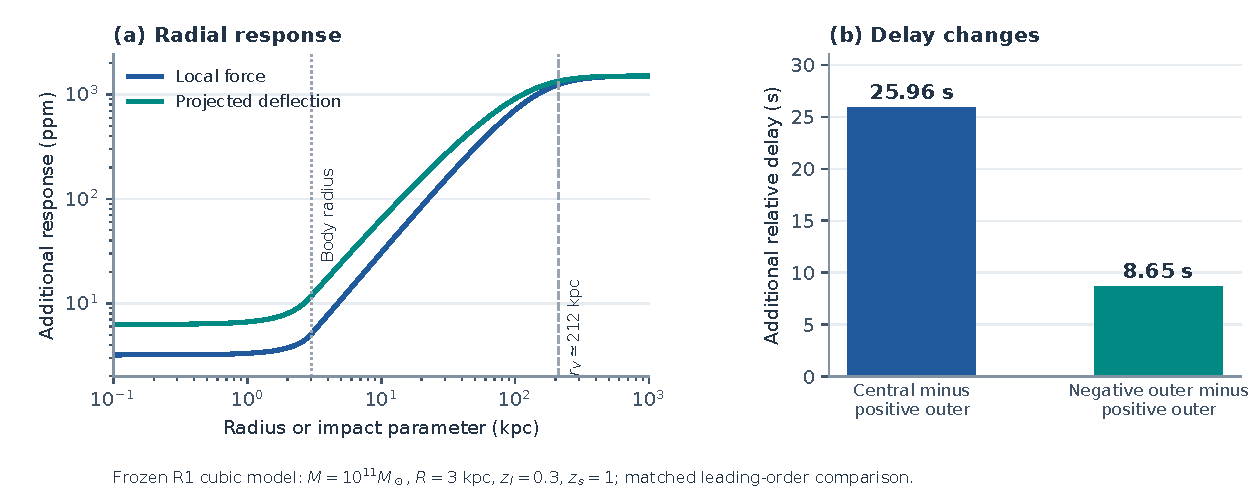
\includegraphics[width=\linewidth]{figures/r1_screening_prediction.pdf}
 \caption{R1 envelope response relative to the fixed-body reference. Left:
 additional local force and projected deflection as fractions of their
 fixed-body reference values. The distinction reflects integration along the
 ray. Right: reference-relative offsets in the two delays for the fixed source
 preparation. Neither panel is an observational detection forecast.}
 \label{fig:prediction}
\end{figure}

At fixed epoch, $r_V\propto M^{1/3}$. The same frozen background also
specifies the redshift dependence, without refitting:
\begin{center}
 \begin{tabular}{rrr}
 \toprule
 Lens redshift & $\epsilon_\infty$ & $r_V$ (kpc), $M=10^{11}M_\odot$\\
 \midrule
 $0.0$ & $0.00351132$ & $248.300$\\
 $0.3$ & $0.00150789$ & $212.029$\\
 $0.5$ & $0.00086052$ & $191.230$\\
 $1.0$ & $0.00022832$ & $150.778$\\
 $1.5$ & $0.00007085$ & $123.011$\\
 \bottomrule
 \end{tabular}
\end{center}
This is a prediction for the coefficients and force law, not a delay
table for identical angular sources at these different redshifts.

The supplied reference-run outputs give the following implementation checks.
The integrated scalar flux has maximum relative residual
$7.9\times10^{-16}$. A direct line-of-sight quadrature and an independent
angular-substitution quadrature agree on the additional deflection to
$4.5\times10^{-13}$ relative. The image equation residual is below
$8.5\times10^{-22}$ rad. Differentiating the projected potential and
deflection independently gives relative discrepancies below
$2.0\times10^{-9}$ and $2.4\times10^{-12}$, respectively.
Finite re-solved and stationary first-order delay changes differ by
$0.00016$ s and $0.000056$ s. These are numerical and perturbative checks
within the model, not bounds on omitted physics. In the current Windows
replay, the corresponding flux residual is $8.30\times10^{-16}$ and the
deflection-derivative discrepancy is $3.19\times10^{-12}$; the remaining
differences are recorded with their numerical tolerances in the replay
receipt. The supplied and replay outputs remain separate records.

\section{Conventional Representation and Consistency Checks}
\label{sec:degeneracies}
\subsection{Positive effective-mass representation of the same response}
The retained metric and optical response admit an explicit conventional
representation. Define an effective additional enclosed mass by
\begin{equation}
 \delta M_{\rm eff}(r)=M f_M(r)F(r),\qquad
 \delta\rho_{\rm eff}(r)=
 \frac{M}{4\pi r^2}\frac{\dd}{\dd r}[f_M(r)F(r)] .
 \label{eq:halo}
\end{equation}
This density is nonnegative. To see this, put
$S=\sqrt{1+r_V^3f_M/r^3}$ and
$n_M=\dd\ln f_M/\dd\ln r\ge0$. Then
\begin{equation}
 \frac{\dd\ln(f_MF)}{\dd\ln r}
 =\frac12\left[(1+S^{-1})n_M+3(1-S^{-1})\right]\ge0 .
 \label{eq:positive-halo}
\end{equation}
The ordinary Poisson field of
$M(<r)+\delta M_{\rm eff}(r)$ has exactly the same $\Phi=\Psi$
as Equation~\eqref{eq:force} within the retained approximation.
It therefore reproduces the full deflection field, relative potential,
images and delays, including multiple source planes in the same geometry.
Its asymptotic extra mass is
\begin{equation}
 \delta M_{\rm eff}(\infty)=\epsilon_\infty M
 =1.50788624\times10^8M_\odot .
 \label{eq:halo-total}
\end{equation}

The rank-one multiple-source residual discussed below distinguishes the scalar from the
restricted Tolman--VII parameter family, not from all conventional
matter distributions. Because slow matter and light respond to the same
retained potentials, ordinary dynamical data do not automatically break
this equivalence either. Independent restrictions on the matter/environment model or an observable
outside this retained equivalence would be needed to distinguish those
representations. No such independent likelihood is asserted here, and
such a distinction is not required for the envelope-transfer calculation.

The effective mass in Equation~\eqref{eq:halo} represents the same
retained contribution as the scalar correction in
Equation~\eqref{eq:force}. One uses either the explicit scalar correction
or its effective-mass representation in the encounter, not their sum.
The construction proves equivalence of the retained metric and optical
response. It does not yet derive both descriptions from one normalized
microscopic BHSM surface source. That common-source derivation remains
open without changing the framework organizing the calculation.

\subsection{The ordinary finite-body control}
For the conventional control, a regular Einstein-fluid interior can be
matched to Schwarzschild. Its compactness is
$m_g/R=1.59514\times10^{-6}$.
The leading optical application above uses the weak-field projection of
this density.

\subsection{A common second-order ordinary-gravity control}
\label{sec:gr2-method}
To test the effect of the first omitted conventional deflection, we
expand the exact static GR optical scattering integral of the same
Tolman--VII body through second post-Minkowskian order (2PM).
Put $\varepsilon_g=m_g/R$, $y=b_{\rm imp}/R$ and
$t=\sqrt{1-y^2}$. The additional radial deflection is
\begin{align}
 \delta\hat\alpha_{\rm GR2}(b_{\rm imp})&=2\varepsilon_g^2 I(y),
 \label{eq:gr2-alpha}\\
 I(y)&=\begin{cases}
 \displaystyle\frac{15(\arcsin y-yt)}{4y^2}
 +y\left(\frac{15}{2}t-4t^5-\frac{48}{7}t^7\right),&0<y<1,\\[4pt]
 \displaystyle\frac{15\pi}{8y^2},&y\ge1.
 \end{cases}
 \label{eq:gr2-I}
\end{align}
At the center $I(0)=0$ and $I'(0)=-6/7$; the interior coefficient
includes the leading fluid pressure and the conversion from areal radius
to invariant asymptotic impact. At and outside the surface it matches the
standard $15\pi m_g^2/(4b_{\rm imp}^2)$ exterior deflection
\citep{IyerPetters2007}.
The consistent plane potential is
\begin{equation}
 \delta\hat\psi_{\rm GR2}(b_{\rm imp})
 =2\varepsilon_g^2R J(y),\qquad J'(y)=I(y),\qquad J(1)=0.
 \label{eq:gr2-potential}
\end{equation}
The supplied implementation evaluates $I$, $I'$ and $J$ analytically.

The R1 response and fixed-body reference receive the identical GR2 potential,
gradient and Hessian, and both image systems are re-solved. The R1
coefficients and leading scalar profile are held fixed. The scattering
impact is identified with the physical thin-plane impact in this control.
This checks robustness to the common GR term; it does not compute the
missing scalar--GR higher-order terms or a complete finite-distance 2PM
cosmological arrival functional. The replay command is
\begin{quote}\small\ttfamily\raggedright
python scripts/run\_strong\_lensing\_gr2\_control.py
\end{quote}

\subsection{Result of the common GR correction}
\label{sec:gr2-result}
At the original two exterior-image impacts, the GR2 term is $3.68$ and
$4.68$ ppm of the leading conventional deflection. Its inclusion changes
the conventional image coordinates by
$(+1.35456,-0.01519,-1.72123)$ microarcsec and the conventional
relative delays by $(+8.28473,+2.55245)$ s.
The absolute correction is therefore material at the scale of the
calculated reference-relative image shifts.

The response-minus-fixed-body-reference offsets are considerably more
stable under this common-term check.

\begin{table}[htbp]
 \centering
 \caption{Robustness of the reference-relative R1 offsets under
 the same GR2 correction in both calculations. The final column is the change
 in the reference-relative offset, not the absolute GR correction.}
 \label{tab:gr2-control}
 \begin{tabular}{lrrr}
 \toprule
 Response offset & Leading calculation & Common GR2 added & Change\\
 \midrule
 $\delta\Delta t_{10}$ (s) & $25.95925815$ & $25.95932714$ & $+68.99\ \mu$s\\
 $\delta\Delta t_{20}$ (s) & $8.64901938$ & $8.64900924$ & $-10.14\ \mu$s\\
 $\delta\theta_0$ ($\mu$as) & $+6.12327625$ & $+6.12326934$ & $-6.91\times10^{-6}\ \mu$as\\
 $\delta\theta_1$ ($\mu$as) & $+0.78810716$ & $+0.78810711$ & $-5.58\times10^{-8}\ \mu$as\\
 $\delta\theta_2$ ($\mu$as) & $-4.34859153$ & $-4.34858643$ & $+5.09\times10^{-6}\ \mu$as\\
 \bottomrule
 \end{tabular}
\end{table}

The two relative changes in the reference-relative delay offsets are
$+2.66$ and $-1.17$ ppm. The delay-ratio response remains $6.8212$ ppm.
Thus the nonzero reference-relative response survives this specific common-term
control without changing its quoted precision in seconds or microarcseconds.

An independent mixed stationary-action derivative reproduces the change
in the reference-relative delay offsets within $0.7$ ns; this checks the small
drift without subtracting four re-solved delays.

The analytic correction was also compared with direct null-geodesic
scattering in the solved static GR fluid and exterior metric. At the
three reference impacts, the exact deflection minus the 1PM and 2PM
terms has magnitude below $1.8\times10^{-16}$ rad for this body's
compactness $\varepsilon_g=1.59514\times10^{-6}$.
A compactness extrapolation independently recovers the interior 2PM
coefficient, and direct integration verifies $J'=I$.
The latter checks establish the implemented ordinary-GR scattering
coefficient, not a physical error bound for the scalar model or its
cosmological embedding. The full corrected coordinates, delays and
checks are supplied in \texttt{gr2\_control.json} and the review outputs.

\subsection{Single-source constraints and nuisance freedoms}
For an observable residual $\delta y=y-y_0$, write
\begin{equation}
 \delta y=B\,\delta a+N\,\delta\nu+\epsilon,\qquad
 W\mathsf C W^T=I,\qquad
 P=I-(WN)(WN)^+ .
 \label{eq:nuisance}
\end{equation}
Here $B$ is a physical response, $N$ the stated nuisance response,
$\mathsf C$ a specified covariance, and $+$ a Moore--Penrose inverse.
The rank of $PWB$ concerns distinguishability in that nuisance model.
A zero direction is unconstrained by the corresponding likelihood; a
Fisher pseudoinverse does not turn it into a zero error bar.
We take $\mathsf C$ positive definite. For the screened comparison,
the single column is a fixed reference-relative response template; rank one denotes
a surviving residual direction, not identification of a freely varied
fundamental scalar parameter.

Using source position, body mass and radius, and a compensated mass-sheet
scale as nuisances, the single R1-response column has projected rank
one if the body center is fixed. Adding both center coordinates gives
rank zero. The raw delay shifts in Table~\ref{tab:delays} are therefore not
nuisance-independent observables for this configuration.
The rank calculation uses $0.001$ arcsec and $0.1$ day as numerical
whitening scales, not as demonstrated observational precisions.

The ordinary mass-sheet transformation,
\begin{equation}
 \psi_\lambda(\theta)=\lambda\psi(\theta)
       +\frac{1-\lambda}{2}|\theta|^2,\qquad
 \beta_\lambda=\lambda\beta,\qquad
 \Delta t_\lambda=\lambda\Delta t ,
 \label{eq:mst}
\end{equation}
cancels from the ratio of two delays. It does not remove source,
centering, radial-profile, or independent line-of-sight freedoms
\citep{Teodori2022}. Consequently the $6.8212$ ppm ratio change is a
fixed-preparation prediction, not a unique diagnostic of a distinct representation.

For the separately computed axial smooth-map response, the images of a
softened isothermal model depend only on
$\beta=s/D_{os}$, $\theta_E=b_{\rm phys}D_{ls}/D_{os}$, and
$\theta_c=r_c/D_{ol}$, while all delays share the factor
$(1+z_l)D_{ol}D_{os}/(cD_{ls})$. Varying the three scalar maps can therefore
be reproduced by these source/profile changes and a delay scale.
The saved six-anchor response accordingly has zero projected rank in
the unrestricted nuisance model. This analytic factorization concerns
that family; it is not a universal theorem that cosmological lensing
information always vanishes.

\subsection{A bounded multiple-source test}
A supplemental design uses one body and three sources at
$z_s=(0.8,1.2,1.8)$, with source offsets $0.1\theta_{E,s}$ at angles
$(0.15,1.1,2.2)$ rad. These choices were fixed before applying the
screened response. The nuisance model includes independent source
positions and delay scales, a shared mass, radius and center, and
shared physical convergence and two shear components.
The resulting scalar column retains rank one; adding independent
source-plane convergence columns leaves rank one as well.

This surviving component is small: its norm is $0.1202\%$ of the raw
whitened response in the expanded nuisance model. In the same illustrative
weighting, the residual coordinates reach approximately $6$ nanoarcsec
and the residual delays $0.086$ s. The explicit 24 observable weights and
response arrays are supplied with the code.
These tidal nuisance fields are phenomenological controls. This test
does not solve the nonlinear scalar equation for a nonspherical galaxy
and its environment, and it is not a signal-to-noise forecast. Its rank
is specific to the finite radial profile family.

\section{Computational Methods and Reproducibility}
The calculation uses the fixed manuscript source revision
\texttt{49a1dab} and records full input hashes.
The main reproduction command from the repository root is
\begin{quote}\small\ttfamily
python scripts/run\_strong\_lensing\_r1\_screened.py
\end{quote}
The coefficient, independent projection, and multiple-source checks are
under \path{scripts/r1_screened_review/}. Numerical results and their
units are under
\path{artifacts/strong_lensing_r1_screened_20261020/}.
The research package additions and exact commands are integrated with the
pinned repository background and optical dependencies. The recorded
package-era replay of three portable review scripts reproduced all 305
saved numerical values in that environment. The current integration
replayed nine numerical commands, compared 1161 saved numerical values,
and passed 16 focused checks without changing the original numerical
artifacts. These are separate execution records, not independent
physical measurements.
The reproducibility manifest identifies versions and hashes rather than
equating successful execution with physical validation.

OpenAI ChatGPT and Codex materially assisted derivation, code development,
numerical checks, interpretation and manuscript revision. The independent
quadrature uses the same physical radial equation but a separately
implemented integration variable and root calculation. Its agreement is a
reproducibility check, not independent empirical evidence or external
human peer review.

\section{Discussion: BHSM Interpretation, Accuracy and Remaining Derivation}
\label{sec:discussion}
The calculation supplies a nonzero local response with an amplitude
fixed by the stated action and background. The known cubic screening
mechanism is not itself new. The specific contribution is its evaluated
finite-body envelope transfer in this reference branch, a consistent
common incident-light comparison, and a constructive conventional
representation of the retained response. The adopted BHSM premise places
those descriptions within the same surface-contribution program; the
calculation establishes their retained optical equivalence while leaving
the normalized microscopic common-source map unfinished.

The numerical precision must be separated from physical accuracy.
The evaluated response and fixed-body reference use leading weak-field,
thin-lens equations. Sections~\ref{sec:gr2-method} and~\ref{sec:gr2-result} explicitly
address the common ordinary-GR second-order term. Its effect on the
absolute image coordinates reaches $1.72$ microarcsec, but its effect on
the offset from the fixed-body reference is below $7\times10^{-6}$ microarcsec.
The two delay differences change by less than $0.1$ ms.
This successful control does not establish absolute microarcsecond
astrometric accuracy or an equivalent physical time-delay error bound.
The scalar--GR mixed terms, scalar corrections to the higher-order fluid
geometry, and finite-distance cosmological 2PM arrival terms remain
uncalculated. The exact effective-halo equivalence in
Section~\ref{sec:degeneracies} is established at the retained leading
scalar order; this common-term test neither extends that proof to all
orders nor changes its retained-order scope.

The scale separation $H_lr_V/c=5.64\times10^{-5}$ supports a local
quasi-static treatment. In the formal isolated projection the contribution
to the extra deflection beyond $20$ Mpc is about
$1.1$--$1.7\times10^{-6}$ of that extra deflection.
Neither check bounds environmental, finite-distance, global matching,
or omitted-sector errors. The reference is spherical; external matter,
time dependence, a finite source, plasma propagation and microlensing
would require additional physical modeling before comparison with data.
The central image is included in the mathematical census; its
detectability is not assumed.
For a nonzero environmental scalar, the cubic equation also contains
mixed local/environmental Hessian terms. Adding an optical tide alone
does not solve that modified local scalar boundary problem.

The leading scalar principal coefficients are positive on the retained
regular branch, as detailed in Appendix~\ref{app:principal}.
However, the radial scalar characteristic speed squared reaches
approximately $1.474$ in units of the metric light speed squared.
This is a property of the scalar effective theory, while the photons used
here propagate on metric null rays. Positive leading coefficients do not
prove complete stability or a causal ultraviolet completion.

The pure cubic specialization does not establish the normalization or
irrelevance of an additional short-distance topographic operator.
A low-momentum expansion with a spatial fourth-order term cannot be
extrapolated to galaxy scales without its coefficient and validity range.
Independent cap/scalar reactions, the general map from exported
topographic forcing into a target phase, and global closed-cosmology
matching remain open. They do not authorize an arbitrary local lensing
amplitude. The constant-target result and the present rolling-scalar
calculation remain distinct conditional sectors.

Appendix~\ref{app:continuation} derives the exact bulk current balance,
its rolling-reference obstruction, the environmental cross-Hessian and
the material/outer-domain conditions consumed by the next application.
These equations do not constitute an evolved higher-order solution.

The next BHSM derivation is therefore specific: reduce the surface,
cap and topographic boundary contributions in the same physical variables
to a normalized source and operator for the independent R1 scalar and
its metric constraints. The reduction must specify the boundary/state
prescription and the complement spectrum or cutoff that controls any
higher-derivative expansion. It must also connect the local response to
the surrounding closed geometry. Neither identifying the rolling scalar
with the target phase or metric coordinate, nor adding an adjustable
optical amplitude, supplies that relation. The present effective
calculation is the evaluated transfer problem to which that derivation
must connect.

\section{Conclusions}
For the prescribed $10^{11}M_\odot$, $3$ kpc body at $z_l=0.3$ and the
common source at $z_s=1$, the conditional cubic R1 envelope calculation gives
offsets in the relative delays of approximately $25.96$ s and $8.65$ s, image changes
of approximately $0.79$--$6.12$ microarcsec, and a $6.82$ ppm change in
the delay ratio. The screening radius is approximately $212$ kpc.
These are reproducible offsets from the fixed-body reference in the declared
leading-order calculation,
obtained without fitting a new scalar amplitude. Adding the same finite-body
GR2 correction to both calculations changes the delay differences by only
$+69$ and $-10$ microseconds in the stated thin-plane control.

The linearized single-source response is absorbed by the admitted source, mass,
radius, mass-sheet and center freedoms. A three-source finite-profile
comparison retains a small shape response, but a positive conventional
effective halo reproduces the entire retained scalar optical field.
Thus prepared light measures the envelope transfer, while the stated
nuisance model controls which properties can be assigned separately. The
positive effective-mass construction is a constructive result: fully
matched conventional and scalar representations share the demonstrated
leading optical response. The source application and positive-complement
construction determine the consumed source relation and prove that its
microscopic completion is not selected by the leading coefficients.
A physical cap-to-$T$ embedding and the specified material/global state
are needed to place this effective calculation within a complete
common-source construction.

\supplementary{The integrated research package contains the local-action
derivation, numerical outputs, independent projection and nuisance checks,
the common GR2 control, source manifests, and exact reproduction commands. The historical
transport and target-sector derivations remain in the pinned repository.}
\authorcontributions{Norman P. Carberry: conceptualization, methodology,
software, validation, formal analysis, investigation, resources, data
curation, writing---original draft preparation, writing---review and
editing, and visualization. The author accepts responsibility for the
scientific content. AI assistance is disclosed below.}
\funding{This research received no external funding.}
\institutionalreview{Not applicable. This theoretical study involves
no human participants or animals.}
\informedconsent{Not applicable.}
\dataavailability{The numerical code, frozen inputs, outputs, source
applications and derivation checks are archived in the public repository
at calculation revision \texttt{0a329fa13f6c} in the
\href{https://github.com/ncarberry64/Manuscript-Generation/tree/0a329fa13f6c90bb2e3b5999b0155aa1e81fe8bd}{Manuscript-Generation calculation archive}.
The frozen background and prior controls are preserved from revision
\texttt{49a1dab}. The accompanying manuscript sources, official journal
dependencies and integration reviews are supplied with this manuscript.}
\acknowledgments{OpenAI ChatGPT and
OpenAI Codex materially assisted mathematical derivation, code generation
and revision, numerical verification, analysis, and manuscript drafting.
The supplied package records its ChatGPT assistance under the label
``GPT-6 Astra Pro'' in its archived validation record. Scientific claims
are specified by explicit equations, executable code and recorded numerical
checks. AI output is not independent scientific evidence. Responsibility
for the content remains with the listed author.}
\conflictsofinterest{The author declares no conflicts of interest.}
\appendixtitles{yes}
\appendixstart
\appendix
\section{The Constant-Target Null Control}
\label{app:target}
The earlier source-free target sector has
\begin{equation}
 S_\eta=-\int N\sqrt h\,w_0 F(X)\,\dd t\,\dd^3x,\qquad
 F(X)=\frac{\kappa_\eta}{2}X+\frac18X^4,\qquad
 X=g^{\mu\nu}\langle D_\mu\eta,D_\nu\eta\rangle ,
\end{equation}
with $\eta=(s,z)\in S^6\subset\mathbb R\oplus\mathbb C^3$,
$s^2+2z^\dagger z=1$, target metric
$\dd s^2+2\operatorname{Re}(\dd z^\dagger\dd z)$, and
$w_0\kappa_\eta>0$. For
$\eta_q=(\cos q,\sin q\,e_1/\sqrt2)$ with constant $q$ and zero
connection, $D\eta=0$, $F(0)=0$, and the target current and stress vanish.
For a radial meridian $q(r)$, regularity sets the conserved flux
\begin{equation}
 r^2e^\nu\sqrt{f_r}\,w_0(\kappa_\eta+X^3)q'=0,
 \qquad X=f_r(q')^2
\end{equation}
to zero. Positivity gives $q'=0$. This proves the null only for the stated
source-free regular boundary problem.

A constant background still permits positive perturbation stiffness.
For a nonconstant Dirichlet phase perturbation, the quadratic energy
and its second variation (phase self-curvature) are
\[
 \begin{aligned}
 E_\eta^{(2)}[\varphi]&=\tfrac12w_0\kappa_\eta
   \int e^{\Phi-\Psi}|\nabla\varphi|^2\,\dd^3x,\\
 \delta^2E_\eta[\varphi,\varphi]&=2E_\eta^{(2)}[\varphi]>0.
 \end{aligned}
\]
The mixed metric/phase response vanishes at $D\eta=0$.
The solved matter body therefore has ordinary nonzero lensing and zero
additional response in this target family. A vanishing matched seam
contribution is not a statement that all possible gravitational or
boundary sources vanish. The rolling scalar $T$ in
Equation~\eqref{eq:r1-action} is a different explicitly specified field.

\section{Moving Measured-Redshift Endpoints}
\label{app:endpoints}
For an observer-normalized affine ray,
$J_a''=\mathcal T J_a$ with
$(J_a,J_a')_a=(0,\omega_a I)$.
Let $Z_{\lambda,a}=\delta\ln\omega|_{\lambda_a}$ and
$Z_{\chi,a}=\delta\ln\omega|_{\chi_a}$. On the reference ray,
\begin{align}
 Z_{\chi,a}&=Z_{\lambda,a}
 -\mathcal H_a\delta\chi_{{\rm ray},a}|_\lambda,\nonumber\\
 \delta\lambda_a&=-\frac{Z_{\lambda,a}}
 {(\ln\overline\omega)'_{\lambda,a}},\qquad
 \delta\chi_a=\delta\chi_{{\rm ray},a}|_\lambda
 +\overline\chi'_{\lambda,a}\delta\lambda_a
 =-\frac{Z_{\chi,a}}{\mathcal H_a}.
\end{align}
Thus converting an affine shift alone does not give the full radial
event shift. The moving-vertex initial conditions are
\begin{equation}
 \delta J_a|_a=-\omega_aI\,\delta\lambda_a,\qquad
 \delta J_a'|_a=\Delta\omega_a I,\qquad
 \Delta\omega_a=\delta\omega_a|_\lambda+
 \overline\omega'_a\delta\lambda_a .
\end{equation}
At fixed measured redshift and observer normalization,
$\Delta\omega_a=0$. Output event and frame conversions must also be
included. These conventions are needed for the three compatible maps;
they are inactive in the local comparison where the maps are held fixed.

\section{Leading Scalar Principal Coefficients}
\label{app:principal}
After eliminating the leading metric mixing, the homogeneous time
coefficient is
\begin{equation}
 D=1+\frac{12Hv}{\lambda}
 +\frac{6v^4}{\Mpl^2\lambda^2}=4.3962210287 .
\end{equation}
For
$\mathcal S=\sqrt{C^2+16b_TGM(<r)/(\lambda r^3)}$,
the leading local diagonal coefficients are
\begin{equation}
 K_r=\mathcal S,\qquad
 K_\Omega=\mathcal S+\frac12r\mathcal S',\qquad
 K_t=D+\frac32(\mathcal S-C)+\frac12r\mathcal S'.
\end{equation}
Nonnegative density implies
$K_\Omega\ge(\mathcal S^2+3C^2)/(4\mathcal S)>0$.
For this branch $K_t$ is also positive; the frozen homogeneous
ratio is $C/D=0.9642051$. The exterior maximum of $K_r/K_t$
is $1.47366$ at approximately $100.107$ kpc.
These are leading local coefficients. Mixed time--space and
higher weak-field terms, the full coupled spectrum, and an ultraviolet
completion are outside this check.

\section{Exact Bulk Continuation, Environment and Matching}
\label{app:continuation}
The retained action also specifies the next field problem. The field
equations below use $c=\hbar=1$, restoring $c$ in scale comparisons. Its
exact bulk equations can be derived without supplying the unfinished microscopic
surface-to-R1 map. They are distinct from an evolved physical solution
with a specified material law and global state. The full spherical
component derivation is supplied in
\path{docs/strong_lensing_r1_screened_20261020/R1_REMAINING_FIELD_DERIVATION_20261020.md}.

\subsection{The current balance and the rolling reference}
Put $U_\mu=\nabla_\mu T$, $Y=U_\mu U^\mu$,
$\Pi_{\mu\nu}=\nabla_\mu\nabla_\nu T$, $S=\Box T$,
$\mathcal K_\Pi=\Pi_{\mu\nu}U^\mu U^\nu$ and $g_3=2/\lambda$.
The exact metric equation and cubic stress are
\begin{align}
 \Mpl^2G_{\mu\nu}&=T^m_{\mu\nu}+U_\mu U_\nu
             -g_{\mu\nu}(Y/2+V)+T^{(3)}_{\mu\nu},\nonumber\\
 T^{(3)}_{\mu\nu}&=g_3[-S U_\mu U_\nu-g_{\mu\nu}\mathcal K_\Pi
       +2U_{(\mu}\Pi_{\nu)\alpha}U^\alpha].
 \label{eq:continuation-einstein}
\end{align}
Equation~\eqref{eq:scalar-covariant} has the exact current form
\begin{equation}
 J^\mu=U^\mu+g_3(\Pi^{\mu\nu}U_\nu-SU^\mu),\qquad
 \nabla_\mu J^\mu=-\mu^3.
 \label{eq:continuation-current}
\end{equation}
On the homogeneous reference $J^0=-J$ for the positive current in
Equation~\eqref{eq:current}, reproducing its source sign.
For a spherical patch
$ds^2=-N^2dt^2+A^2dr^2+r^2d\Omega^2$, the actual balance is
\begin{equation}
 \partial_t(NAr^2J^t)+\partial_r(NAr^2J^r)=-\mu^3NAr^2.
 \label{eq:continuation-balance}
\end{equation}
An exactly static metric with $T=vt+\pi(r)$ and constant $v$ would remove
the temporal term. A regular center would then require
\begin{equation}
 J^r(r)=-\frac{\mu^3}{NAr^2}\int_0^rN(s)A(s)s^2\,\dd s,
 \label{eq:continuation-static}
\end{equation}
which grows as $-\mu^3r/3$ in a static asymptotically flat region, rather
than giving the decaying isolated excess. Moreover $V_0-\mu^3vt-\mu^3\pi$
makes the stress time dependent for nonzero $\mu^3v$. The rolling
background time-current balance must therefore be retained before its
homogeneous contribution is subtracted. The executed quasi-static
solution does this at its retained order; appending a static GR2 potential
does not solve this full continuation. Small $H_lr_V/c$ supports the
local freezing approximation but is not a physical delay-error bound.

\subsection{The environmental contraction}
At the retained quasi-static order let $\pi_T=\pi_L+\pi_E$ and
$\delta\rho=\rho_L+\rho_E$. Subtracting the environmental equation from
the total scalar equation gives the actual local application
\begin{align}
 C\Delta\pi_L
 &-\frac2\lambda[(\Delta\pi_L)^2-\Pi_L:\Pi_L]\nonumber\\
 &-\frac4\lambda[(\Delta\pi_E)(\Delta\pi_L)-\Pi_E:\Pi_L]
   =-\frac{b_T\rho_L}{2\Mpl^2},
 \label{eq:continuation-environment}
\end{align}
where $\Pi_{L,ij}=\partial_i\partial_j\pi_L$ and similarly for $E$.
The environmental input is the full spatial Hessian in
$[(\operatorname{tr}\Pi_E)\delta^{ij}-\Pi_E^{ij}]
\partial_i\partial_j\pi_L$, not its trace alone. Constant or
uniform-gradient scalar data have no such cross term, whereas a tidal
Hessian generally does. A projected optical tide does not determine this
three-dimensional contraction. Physical environmental density and
boundary/Cauchy data must be solved with the same scalar and metric
constraints; their total principal operator must also be checked.
The optical nuisance tides in the main text do not perform that solve.

\subsection{Material and outer-domain defining data}
An evolved perfect fluid consumes a material relation, for example
$\rho_m=\rho_m(n)$ and $p_m=n\,\dd\rho_m/\dd n-\rho_m$, together with
$\nabla_\mu T_m^{\mu\nu}=0$. At static equilibrium the radial application
is $p_m'=-(\rho_m+p_m)\nu'$ for $N=e^\nu$.
A common fixed barotropic law with $\delta\rho_m=0$ would give
$\delta p_m=0$, whereas Equation~\eqref{eq:pressure} gives a positive
pressure change. The retained comparison therefore prescribes common
density, not a common fixed material equation of state. A physical
material continuation must allow density readjustment, specify additional
support, or explicitly retain the prescribed-stress comparison.

In an overlap worldtube $r_V\ll r_m\ll c/H_l$, the regular branch fixes
its far-zone derivative data without a new local charge:
\begin{align}
 \pi_T'(r_m)&=-\frac{b_TGM}{Cr_m^2}
       [1+O((r_V/r_m)^3)],\nonumber\\
 \Phi'(r_m)=\Psi'(r_m)&=\frac{GM}{r_m^2}
       [1+\epsilon_\infty+O((r_V/r_m)^3)].
 \label{eq:continuation-overlap}
\end{align}
Smooth matching also requires the induced metric and extrinsic curvature,
the scalar value and normal derivative, and the current balance in
Equation~\eqref{eq:continuation-balance}. Scalar additive data and clock
normalization belong to the outer state. A physical surface source would
instead require its variational junction conditions; no moving-seam law
is assumed here.

The flat local constraint cannot be extended unchanged to the entire
compact slice. Its formal compact integral would require
$\int\delta\rho\,\dd V=0$, which the isolated positive excess does not
satisfy. The actual outer problem must retain curvature, time dependence
and the homogeneous response, or a declared compensating excess. This
is a compatibility check of the naive extension, not a prohibition of
positive local mass in a closed cosmology. The outer solution must match
both the local field and the source/observer clock protocol. Thus the
exact bulk and environmental equations are available, while their
material and global state data must be specified before a further
physical solution is claimed.

\section{Common-Source Pullback and a Nonuniqueness Construction}
\label{app:source-reduction}
The original cap reduction is a constrained critical value with retained
boundary traces and kernel coordinates. Its actual matcher variation
defines the oriented canonical momenta by
$\delta S_{5,\epsilon}^{\rm on\mbox{-}shell}
=\int\Pi_\epsilon^{ab}\delta\gamma_{\epsilon ab}$ and
$S_{\rm match}=\sum_\epsilon\int\Lambda_\epsilon^{ab}
(h_{ab}-\gamma_{\epsilon ab})$. It gives
\begin{equation}
 \Pi_\epsilon^{ab}=\Lambda_\epsilon^{ab},\qquad
 2C_\partial G^{ab}[h]=T_m^{ab}+\tau_{\rm cap}^{ab},\qquad
 \tau_{\rm cap}^{ab}=\frac2{\sqrt{-h}}\sum_\epsilon\Pi_\epsilon^{ab}.
 \label{eq:cap-source-pullback}
\end{equation}
Thus $u_a u_b\delta\tau_{\rm cap}^{ab}$ supplies the metric energy
source once a cap solution and observer are specified. The cap scalar
normal momentum and the interface Euler variation supply different
source slots; their pullback into canonical $T$ must be established.
The cap sum cannot be replaced with the reflection-even mean without
its factor of two. A cap response absorbed into the local action is
accounted for once.

For original coupled rows $A_P\psi+Bq=J_P$,
$B^\dagger\psi+D_Qq=J_Q$, elimination on an invertible owned complement
gives both the operator and its forcing:
\begin{equation}
 (A_P-BD_{Q,\perp}^{-1}B^\dagger)\psi
 =J_P-BD_{Q,\perp}^{-1}J_Q-Bq_0,
 \qquad q_0\in\ker D_Q.
 \label{eq:source-schur}
\end{equation}
Kernel compatibility equations remain explicit. A reduced Hessian
alone does not determine this source. The physical embedding of $T$,
its kinetic normalization, cubic vertex and source pairing must agree
under the same reduction.

The leading R1 coefficients do not select a unique complement. To prove
this, take two mathematical spectral lifts on the same ball
$L=10\pi\ell_0$, both real fields regular at zero and Dirichlet at $L$.
The normalized radial modes are
$f_n=\sin(n\pi r/L)/(r\sqrt{2\pi L})$, $n\ge1$,
with $q=p\ell_0^2=(n/10)^2$. Define
\begin{equation}
 H(q)=\begin{pmatrix}(C+1)q&g\sqrt q\\g\sqrt q&M_c^2+q\end{pmatrix},
 \quad K_{\rm time}=\operatorname{diag}(D,1),
 \quad (M_c^2,g)=(1,1)\ \hbox{or}\ (4,2).
 \label{eq:complement-witness}
\end{equation}
Here $M_c,g,q$ are dimensionless; $D$ is the temporal coefficient in
Appendix~\ref{app:principal}. The same retained source is used and the
complement is explicitly unforced for this counterexample. Neither lift
is selected as a microscopic galaxy state. Each complement is positive,
and its reduced kernel is
$Cq+g^2q^2/[M_c^2(M_c^2+q)]>0$ for every owned $q>0$.
Both leading coefficients are exactly $C,D$, yet after normalizing by
$C$ their fourth-order coefficients are
$B/\ell_0^2=1/C=0.2359125661$ and
$1/(4C)=0.05897814152$, with expansion scales
$p\ell_0^2\ll1$ and $p\ell_0^2\ll4$, respectively.
The common unit $\ell_0$ has not been assigned a physical galaxy scale.
This constructive nonuniqueness result identifies missing physical
selection data rather than inferring them from an unavailable array.

A further direct identification can be excluded. The inherited
distributed seam law
$\nabla\cdot\mathbf F_{\rm top}=a\Theta(r-r_\star)/r^2$ with
$F^r_{\rm top}(r_\star)=0$ integrates to
$F^r_{\rm top}=a(1/r-r_\star/r^2)$. Its growing integrated charge
cannot be identified by a constant normalization with the isolated R1
flux, which decays as $r^{-2}$. A different finite-domain export or
nonlocal source map remains possible. The full action/source trail,
including the interface Euler relation, is supplied in
\path{docs/strong_lensing_r1_screened_20261020/BHSM_COMMON_SOURCE_DERIVATION_20261020.md}.
It specifies the physical embedding, constitutive interface density and
boundary prescription needed for a unique further application.
